\subsection{Testbild ohne Belichtung}
Zunächst wurden zwei Bilder einer Identitätskarte mit maximalem Gain und ohne Beleuchtung aufgenommen. Diese sind in den Grafiken \ref{fig::imLight_1} und \ref{fig::imLight_2} ersichtlich.

\begin{figure}[ht]
	\begin{minipage}{0.45\textwidth}
		\centering
		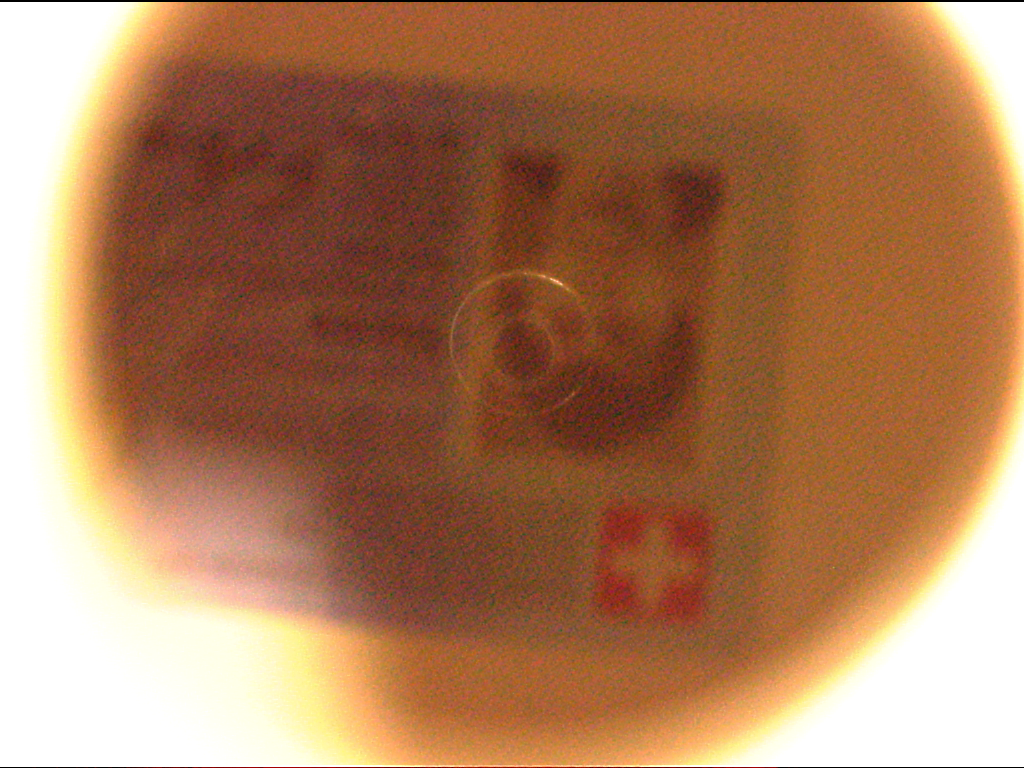
\includegraphics[width=0.8\textwidth]{Posten_4_ID_01.png}
		\caption{Erste Aufnahme der Identitätskarte}
		\label{fig::imLight_1}
	\end{minipage}
	\begin{minipage}{0.45\textwidth}
		\centering
		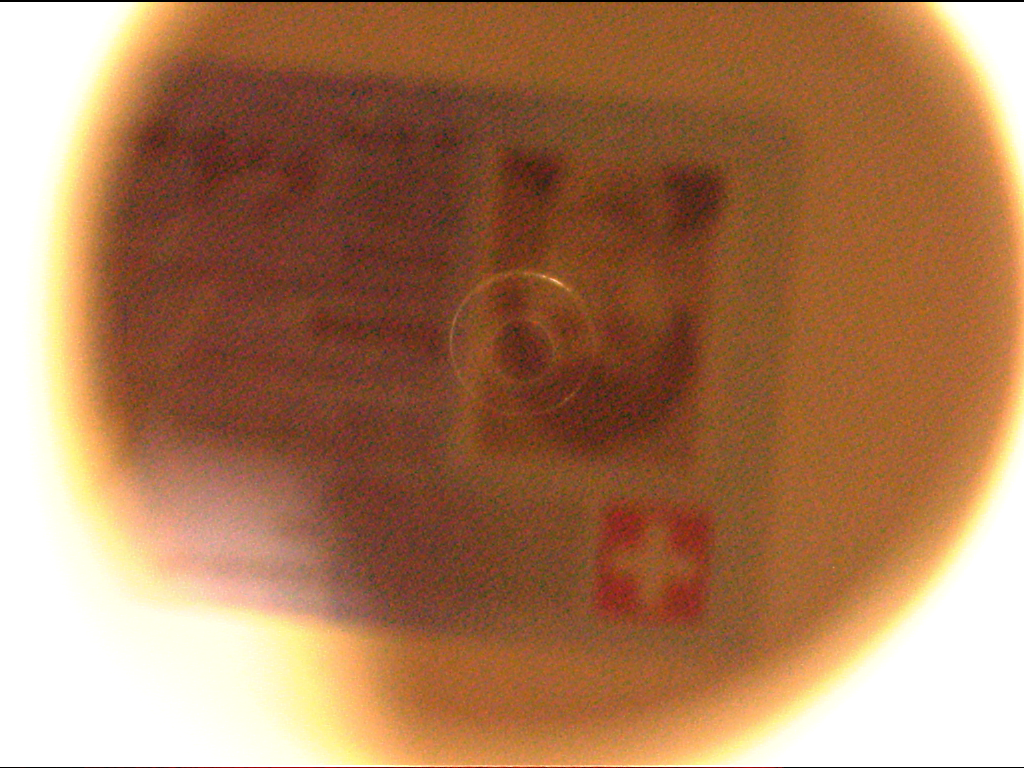
\includegraphics[width=0.8\textwidth]{Posten_4_ID_02.png}
		\caption{Zweite Aufnahme der Identitätskarte}
		\label{fig::imLight_2}
	\end{minipage}
\end{figure}

Es werden nun die beiden Bilder subtrahiert, was das Rauschen ergibt (Grafik \ref{fig::imDiff_1}). Um das Rauschen besser zu sehen wurde dieses um einen Faktor 10 verstärkt (Grafik \ref{fig::imDiff_10}).

\begin{figure}[ht]
	\begin{minipage}{0.45\textwidth}
		\centering
		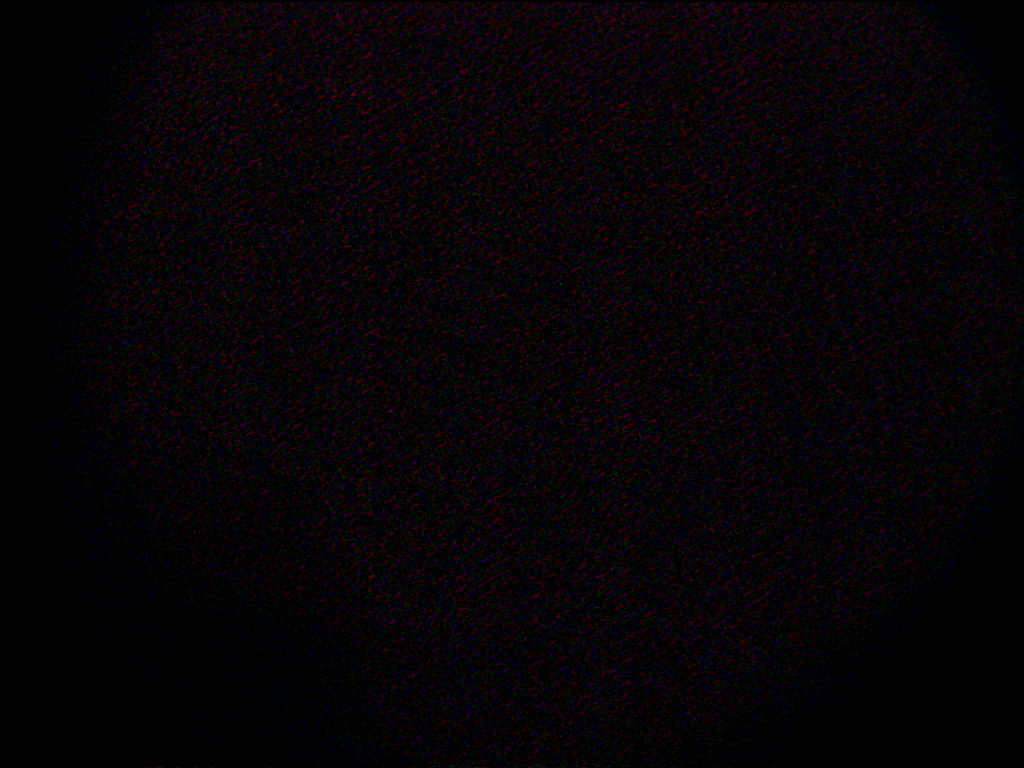
\includegraphics[width=0.8\textwidth]{imDiff_1.png}
		\caption{Unverstärktes Rauschen}
		\label{fig::imDiff_1}
	\end{minipage}
	\begin{minipage}{0.45\textwidth}
		\centering
		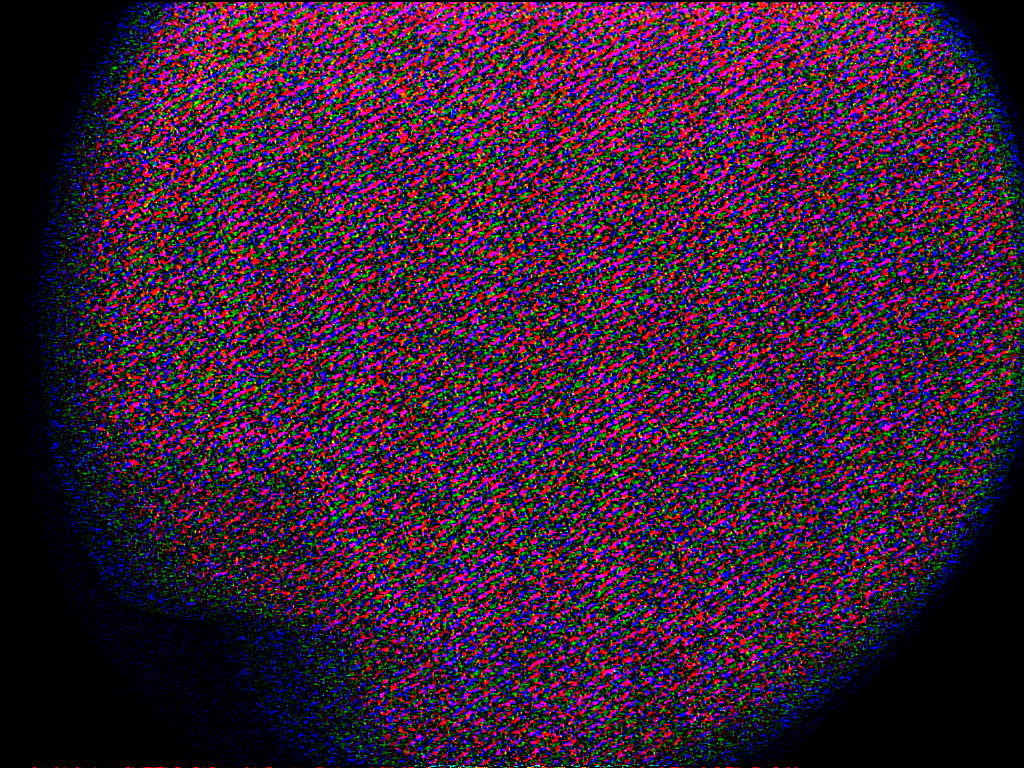
\includegraphics[width=0.8\textwidth]{imDiff_10.png}
		\caption{Verstärktes Rauschen}
		\label{fig::imDiff_10}
	\end{minipage}
\end{figure}

In der Linken Abbildung ist das unverstärkte Rauschen zu sehen, jedoch nur bei genauer Beobachtung. Deshalb wurde dies in der Rechten Abbildung verstärkt, wodurch dies wesentlich besser zu sehen ist. Dadurch ist zu sehen, dass das Rauschen im hellen Bereich des Bildes nicht vorhanden ist. Dies kommt daher, dass die Sensoren der Kamera in diesem Bereich voll ausgesteuert sind was zu einer Differenz von Null zwischen den Bildern führt.
\newpage
\subsection{Schwarzes Testbild}
Weiter wurde eine Aufnahme bei maximalem Gain und minimalen Lichteinfall gemacht, diese Aufnahme ist in Bild \ref{fig::imDead} dargestellt.

\begin{figure}[ht]
	\centering
	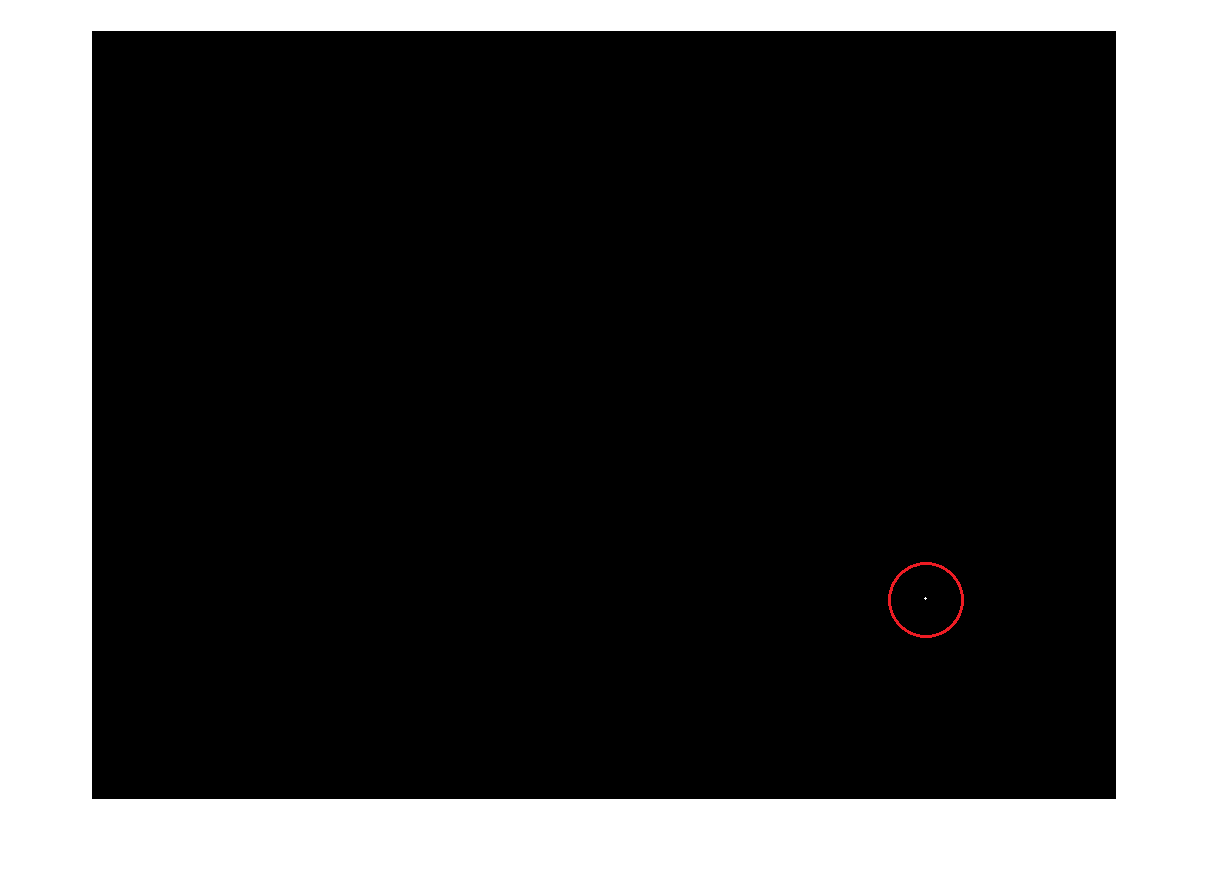
\includegraphics[width=0.8\textwidth]{imDead.png}
	\caption{Aufnahme bei minimalem Lichteinfall}
	\label{fig::imDead}
\end{figure}

In diesem Bild ist in der unteren rechten Ecke (rot markiert) der Pixelfehler der Kamera zu sehen.
\newpage
\subsection{Weisses Testbild}
Als letztes wurde noch eine Aufnahme bei beleuchtetem Dom gemacht (Grafik \ref{fig::imWhite}):

\begin{figure}[!ht]
	\centering
	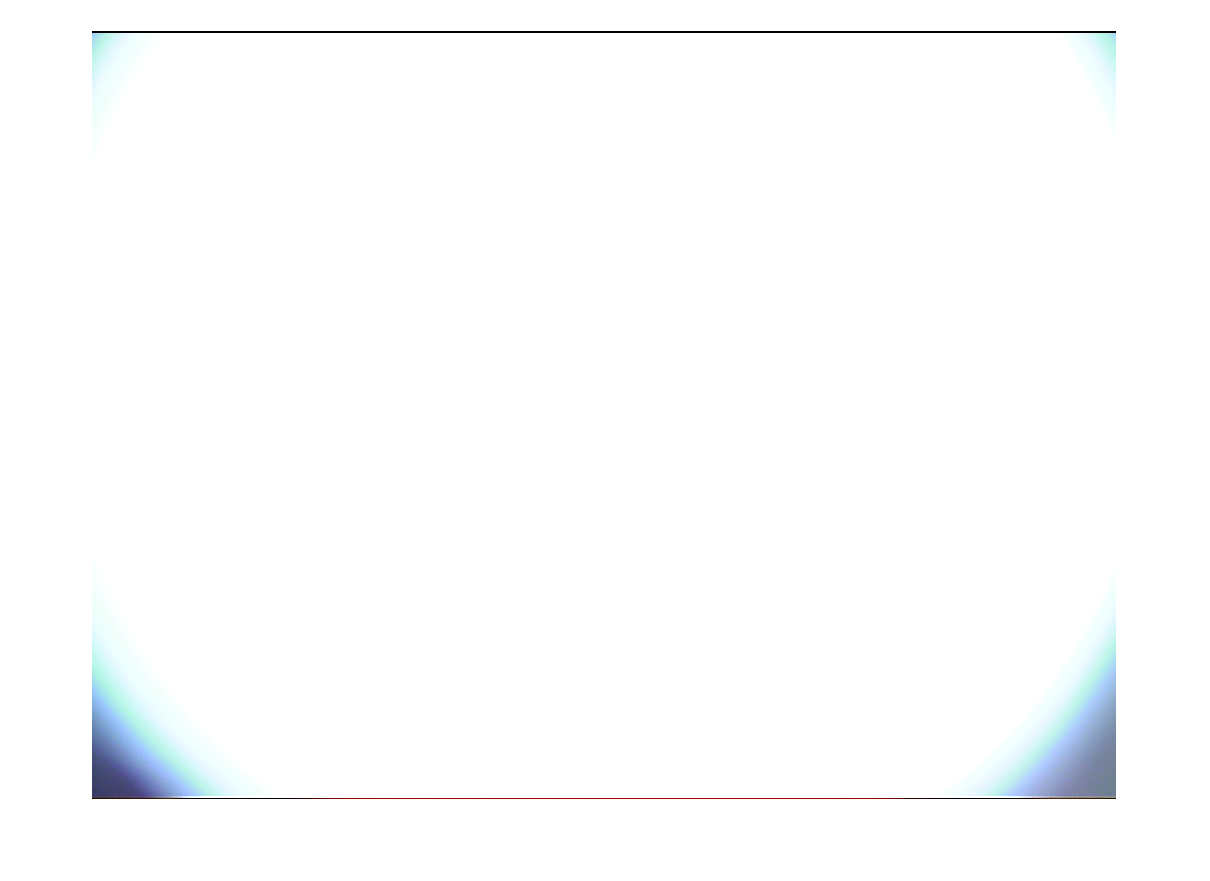
\includegraphics[width=0.8\textwidth]{imWhite.png}
	\caption{Aufnahme bei beleuchtetem Dom}
	\label{fig::imWhite}
\end{figure}

In dieser Aufnahme sollte nun die Vignettierung erkenntlich sein. Die Vignettierung ist in der Grafik jedoch nicht klar ersichtlich, weshalb darauf geschlossen werden kann, dass diese intern entfernt worden ist oder nicht ausgeprägt ist.




